\documentclass[11pt]{article}
\usepackage{graphicx}
\graphicspath{{./Images/}}
\usepackage{setspace}
\usepackage{subcaption}
\usepackage[left=3.2cm, right=3.2cm, top=3cm]{geometry}
\setstretch{1.5}
\begin{document}
\title{Predicting NBA Regular Season Results Based on some popular statistics}
\author{Chenjie Li,Qiao Qiao}
\maketitle
\section*{1.Problem Description}
\subsection*{1.1 Background}
\hspace{1.5em}NBA(National Basketball Association) is one of the most successful basketball league around the world.And since it is popular, there exists tons of websites recording the statistics related to the game. They not only provide simple metrics like Field Goal Percentage,  Average Points, Average Assists, but also some advanced metrics like PER,True shooting percentage and much more.

Based on those statistics, people are exploring what kinds of metrics can result in a team's success or failure as a season.

In this report, we investigated the relationship between the regular season results of the team and some popular metrics in two different perspectives: 
\begin{itemize}
\item \textbf{Players' Effects}:	\textbf{team PER},
\item \textbf{Teams' Overall Effects}: \textbf{Team's Offensive Efficiency}(TOE)
\end{itemize}
) for the past 5 seasons ($2014-2018$).Based on the results we get, we made some predictions for the results of this uocoming season.

\section*{2.Data Source}
\hspace{1.5em}There are many "data hubs" available, our data source is mainly from \\1insider.espn.com/nba/hollinger/statistics and https://www.basketball-reference.com/.

To be able to work with data, we deveoped a "web crawler" using Python Scrapy library. By using the program we got the formatted CSV file so that we can easily input them in R.

Furthermore, since we are familiar with Database and SQL language, we also put the data in a database so we can manipulate the data easily by Queries.
\section*{3.Win Ration Analysis}
\subsection*{3.1Team Offensive Efficieny Analysis}
\subsubsection*{3.1.1 New TOE introduction and Experiments}
\hspace{1.5em}Offensive Efficiency, as the name suggests, is a parameter measuring the efficiency of the offense.Here we explain this intuition by giving an simplified example:

Player A took 5 shots and made 4 of them; Player B took 5 five shots, and made 2 of them. Therefore, we can conlcude that player A is more efficient than Player B.

Of course, this is a oversimplified example.

There are a lot different kinds of definitions for Player and Team's Efficiency:
In Shea,Stephen M's book$^1$, They define the Offensive Efficiency for Team as:
\begin{center}
$TOE = \frac{FG}{FGA \;-\; ORB\; + \;TO}$
\end{center}
Where FG is the field goals made, FGA is the field goals attempts, ORB is the number of offensive rebounds, TO represents the number of turnovers. 

It is of course reasonable to guess that the more efficient a team's offensive is, the more number of games a team is going to win.This idea was proved in their book: "The top 5 teams in OE in the 2012-2013 season all won at least 56 games."

This book was written and published five years ago. As time goes by, NBA statistics has been getting more and more comprehensive.
Now we want to propose a new version of Team's offensive efficiency.

The formula we proposed is:
\begin{center}
$New\;TOE = \frac{2PTM \;+ \;1.5 \;* \;3PTM}{FGA \;-\; ORB \;*\; ORBS\% \; + \;TO\; * \;OP\_POTS\%}$
\end{center}
Where \textit{2PTM}means 2 points field goals made;\textit{3PTM} means 3 points field goals made; \textit{ ORBS\%} means the offensie rebound scoring rate; \textit{OP\_POTS\%} means opponent scoring rate off the team's turnovers.

Now let's motivate our formula. An individual offensive possesion could lead up to 4 possible results: taking a 2 point shot, taking a 3 point shot, missing a shot but getting an offensive rebound, and turning the ball over. We believe a 3 point shot is worth 1.5 2 point shot. Offensive rebound could compensate the results of missing the shot.Since most(not all of them, of course) second chance points are 2 points, we ignored the effect of the 3 point second chance points.but here we times Offensive rebound by "offensive rebound scoring rate", because different teams might have different abilities to convert a offensive rebound to box score.Here we also ignored the effect of 3 points made by opponent off turnovers.And finally, we add a factor "$TO\; * \;OP\_POTS\%$" to take the effects of turnovers into consideration.

In this section all our data is from \textit{https://stats.nba.com/}$^2$.

We calculated the results from Season 2014 - Season 2017, here we only show two groups of results. For comprehensive results, please check out the Appendix part.
\begin{figure}[h!]
  \centering
  \begin{subfigure}[b]{0.45\linewidth}
    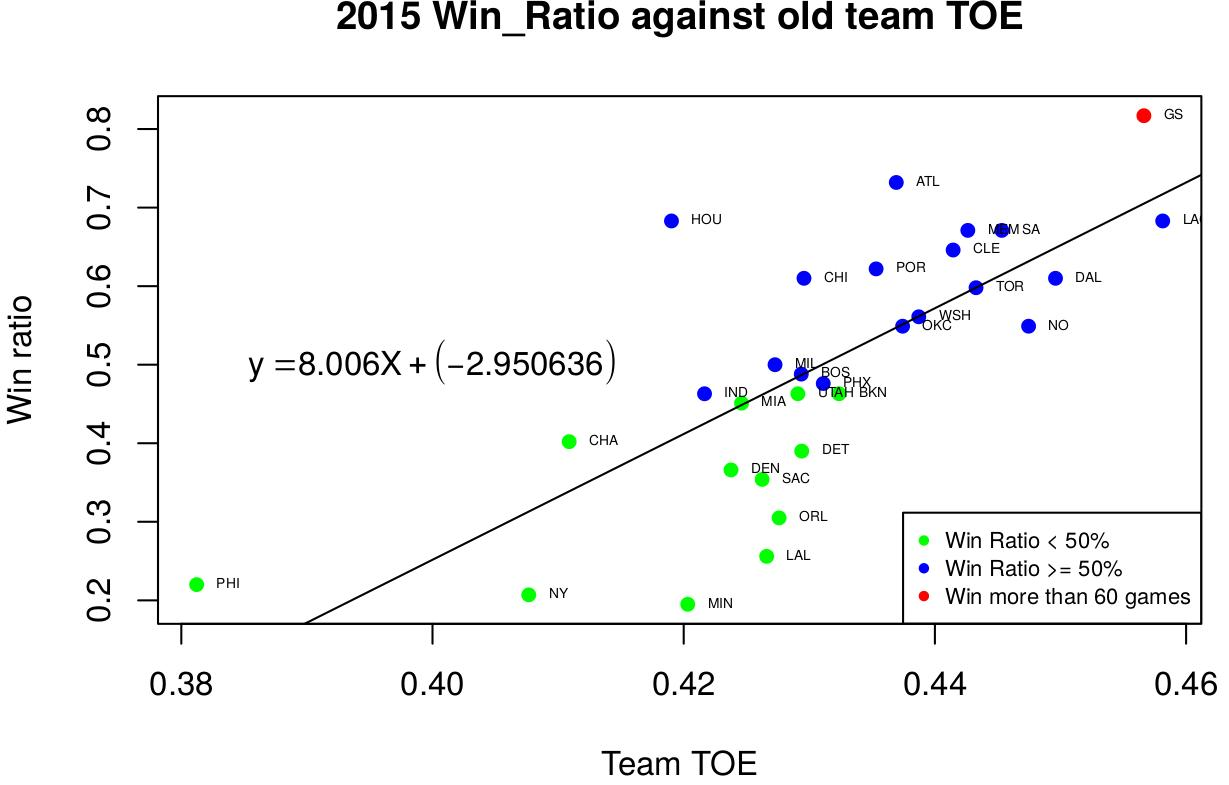
\includegraphics[width=\linewidth]{15old.jpg}
  \end{subfigure}
  \begin{subfigure}[b]{0.45\linewidth}
    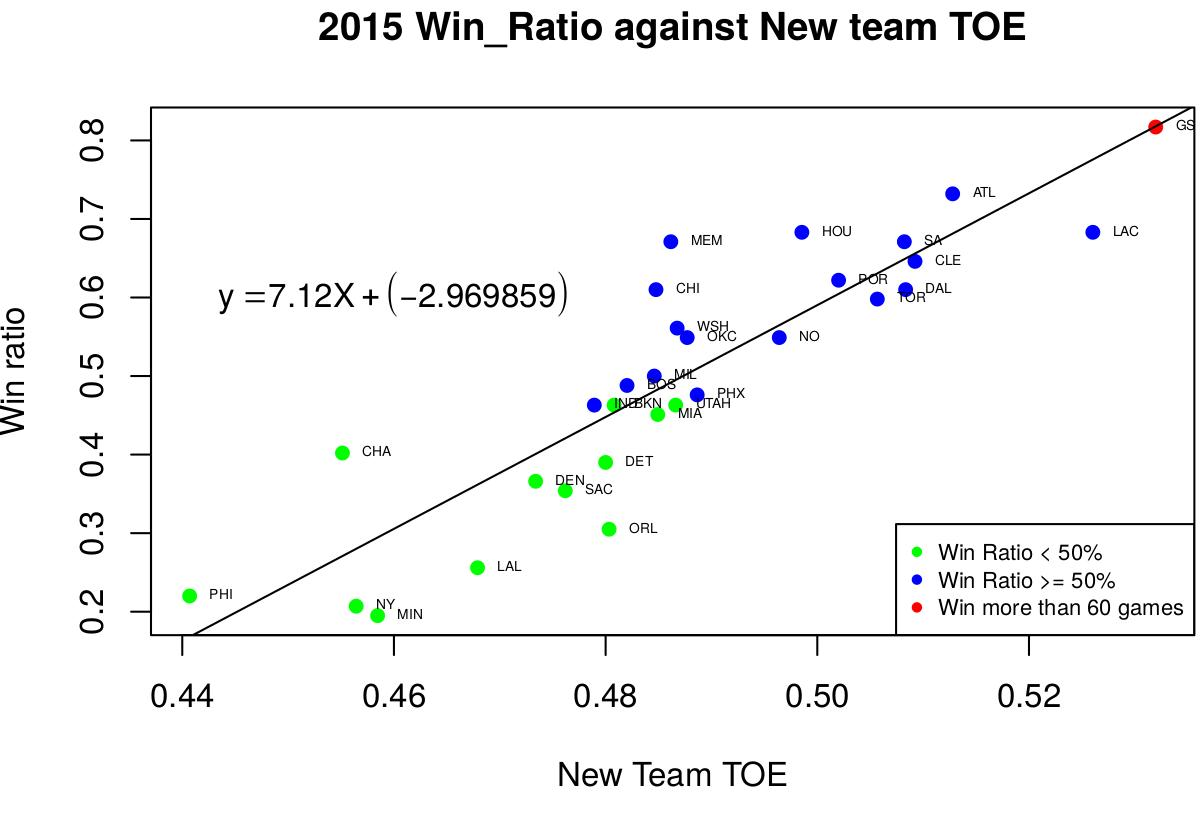
\includegraphics[width=\linewidth]{15new.jpg}
  \end{subfigure}
  \begin{subfigure}[b]{0.42\linewidth}
    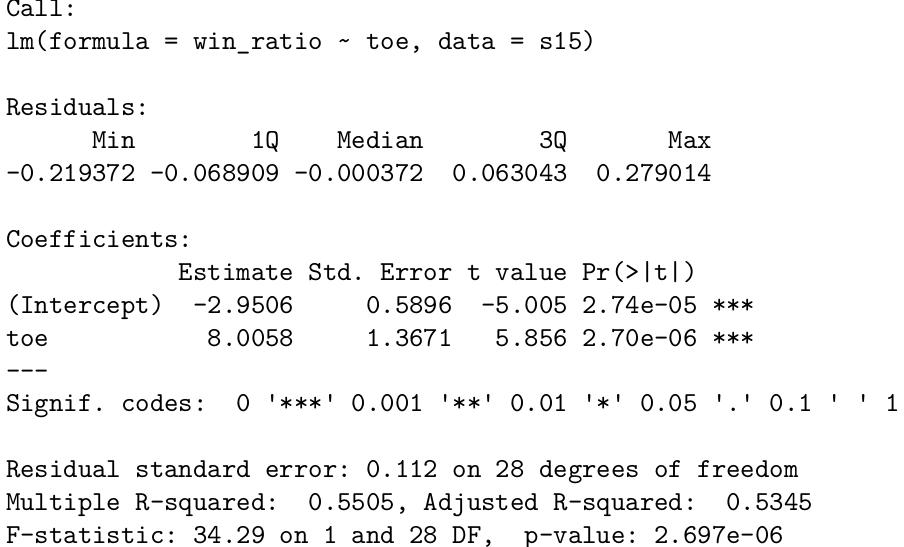
\includegraphics[width=\linewidth]{15oldSummary.jpg}
    \caption{2015 Season Using Old TOE}
  \end{subfigure}
  \begin{subfigure}[b]{0.42\linewidth}
    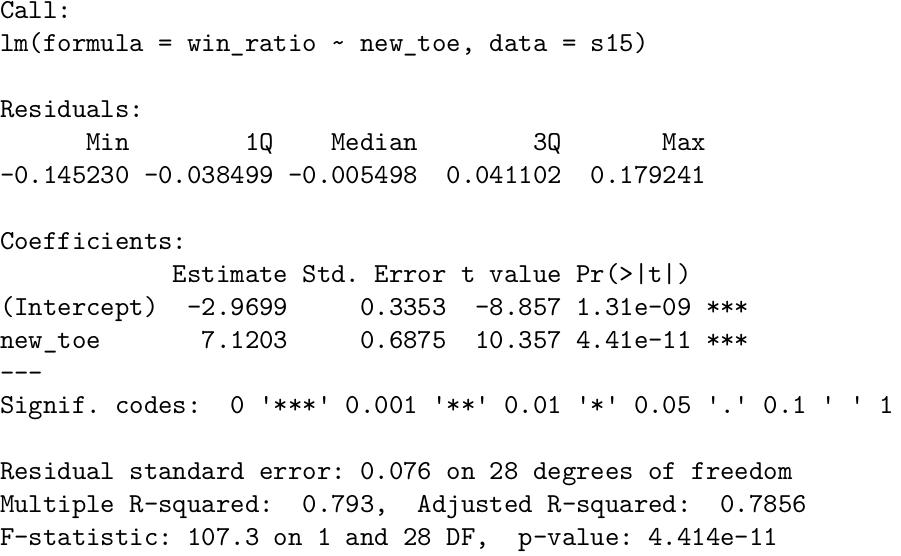
\includegraphics[width=\linewidth]{15newSummary.jpg}
    \caption{2015 Season Using New TOE}
  \end{subfigure}
  \caption{Comparision Between TOE and New TOE in 2015 Season}
\end{figure}
\begin{figure}[h!]
\centering
 \begin{subfigure}[b]{0.4\linewidth}
  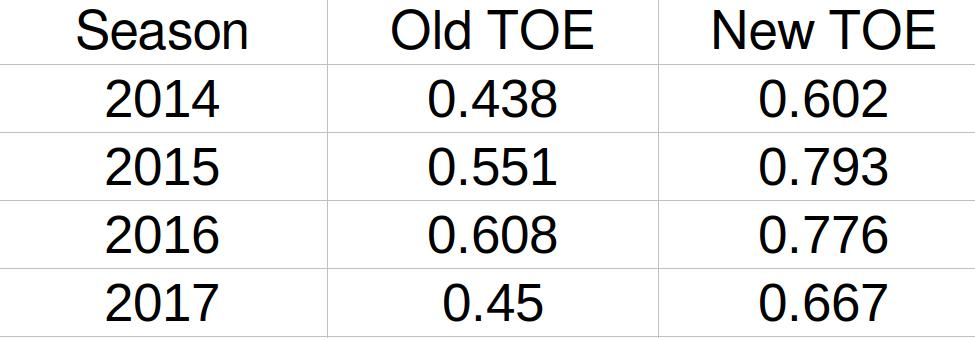
\includegraphics[width=\linewidth]{ComparisionR.jpg}
 \end{subfigure}
 \begin{subfigure}[b]{0.4\linewidth}
  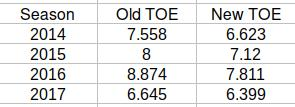
\includegraphics[width =\linewidth]{Beta1.jpg}
\end{subfigure}
 \caption{Comparison of $R^2$(left) and $\beta_1$(right)}
\end{figure}

As Figure 1 and Figure 2 show, our new TOE is much better(significantly higher $R^2$ value) than evaluating the relationship between Win Ratio and Team Offensive Efficiency. We noticed the coefficient $\beta_1$ values keep increasing in 3 consectutive years, whereas in 2017 the $\beta_1$
drops again.

\newpage
\subsubsection*{3.1.2 Prediction}

Now we want to use first four seasons (2014-2017) data combined to make a prediction for season 2018, which has already ended.Our goals is to test how accurate our predictions are compared with the facts.

\newpage
\section*{4. References}
1. Shea, S. M., Baker, C. E. (2013). Basketball analytics: Objective and efficient strategies for understanding how teams win. CreateSpace Independent Pub. Platform.\\
2. Teams General Misc Statistics. Retrieved from \textit{stats.nba.com} 


\end{document}

